\documentclass{comjnl}

\usepackage{amsmath}
\usepackage{amssymb}
\usepackage{bm}

\begin{document}


\title[3-D Keypoint detection with DNNs]{3-D Keypoint detection with Deep Neural Networks,
Sparse Autoencoders and Mesh Simplification}
\author{El\'{i}as Josu\'{e} Puma Ch\'{a}vez}
\affiliation{Escuela Profesional de Ciencia de la Computaci\'{o}n,\\
Universidad Nacional de San Agust\'{i}n,\\
Arequipa, PE}
\email{eliasj.puma@gmail.com}

\shortauthors{El\'{i}as J. Puma}

%\received{00 January 2009}
%\revised{00 Month 2009}


%\category{C.2}{Computer Communication Networks}{Computer Networks}
%\category{C.4}{Performance of Systems}{Analytical Models}
%\category{G.3}{Stochastic Processes}{Queueing Systems}
%\terms{Internet Technologies, E-Commerce}
\keywords{Keypoint detection; Deep Neural Networks; 3-D Model; Sparse Autoencoders}


\begin{abstract}
3-D keypoint detection plays a fundamental role in the Computer Vision field, detection
of these salient points in the local surfaces of a 3-D object is important in order to 
perform certain tasks such as registration, retrieval and simplification. There has been
a lot of research in the field of 3-D keypoint detection, most of them take a geometrical 
approach which have a good performance but lack flexibility to adapt to changes such as
noise and high curvature points that are not keypoints to human preference. A good
approach seems to be machine learning methods that can be trained with human annotated 
training data. In this paper a new method is proposed using deep neural network with 
sparse autoencoder as the regression model due to their great ability for feature processing. 
The analysis shows this method would outperform other methods that are widely used. 
\end{abstract}

\maketitle


\section{Introduction}
Several computer-dependent areas are benefited of the applications
that 3-D Models have in them. The growth of 3-D data has increased in
the last years with the availability of low-cost 3-D capture devices~\cite{harris3D}.
The ability to analyse, proccess and select relevant information
from them is an active research area. 

3-D interest point detection is a difficult task for several reasons~\cite{Discrim, harris3D}.
First, there is not a definition of what exactly a keypoint is, but a common
assumption relates the level of protusion of outstanding local structures
with the measure of interest of such local structure~\cite{harris3D}.
We can say by so, that in planar sections of an area
vertices have a low interest level and in local areas with diferent
structures the interest level will be the opposite, the same with
the edges of an object. Its main caracteristic is its
invariance to transformations in the object itself. Second, vertex 
density is different for every 3-D model which makes harder the task of
selecting a local area. Third, information obtained from a 3-D model
are only vertex positions and connectivity between them which means
the interest level will depend only from the information we can
retrieve from different calculations. These are not the only challenges
to be faced but are sufficient to explain why this method is prepared to
handle these difficulties. 

The common approach to 3-D keypoint detection has been to use 
geometric properties of the models, although in recent years researchers
also have developed machine learning techniques that try to outperform the
former one by avoiding the problems of: Different tasks in different areas
of the model~\cite{DNN}, false positives obtained from noise or local
variation and keypoint detection valuable according to human preference. 

The rest of this paper is organized in the following way:
Section~\ref{RelatedWork} introduces previous work done in the area,
In section~\ref{NeuralNetworkIntro} we explain the basic principles to
build a Deep Neural Network using sparse autoencoders.
Section~\ref{Proposal} presents the idea this method is based on. Future
results will be presented in Section~\ref{Results} and future conclusions
in Section~\ref{Conclusions}.

\section{Related Work} \label{RelatedWork}
In recent years researchers have proposed several techniques for
3-D keypoint detection. Most of them are based on geometric methods,
that work on meshes or use surface reconstruction~\cite{UnstructuredPointCloud}.
Techniques that follow this approach will be introduced below:

Lee~\cite{Lee01} addresses interest point detection through the
use of local curvature estimates together with a center
surround scheme at multiple scales. The total saliency of
a vertex is defined as the sum of Difference of Gaussian
(DoG) operators over all scales.

The THRIFT algorithm~\cite{THRIFT} is a 3-D extension of 2D algorithms
like SIFT and SURF. They divide the spatial space by a uniform voxel grid
and calculate a normalized quantity $D$ for each voxel. To construct a
density scale-space Flint et al. convolve $D$ with a series of 3-D
Gaussian kernels $g(\bm{\sigma})$. This gives rise to a scale-space
$S(\bm{p},\bm{\sigma}) = (D \otimes g(\bm{\sigma}))(\bm{p})$ for each
3-D point $\bm{p}$. Finally, they compute the determinant of Hessian matrix
at each point of the scale space. Within the resulting $3\times3\times3\times3$
matrix, a non maximal suppression reduces the entries to local maxima, which become
interest points.

Mian~\cite{RepeatabilityAndQuality} related the repeatability of keypoints
(extracted from partial views of an object) with a quality measure based
upon principal curvatures. For each point $\bm{p}$ they rotate
the local point cloud neighborhood in order to align its normal vector $n_{\bm{p}}$
to the $z$-axis. To calculate the surface variation they apply a principal
component analysis to the oriented point cloud and use the ratio between the
first two principal axes of the local surface as measure to extract the 3-D keypoints.

Sun~\cite{Sun01} apply the Laplace-Beltrami operator over
the mesh to obtain its Heat Kernel Signature (HKS). The
HKS captures neighborhood structure properties which
are manifested during the heat diffusion process on the
surface model and which are invariant to isometric trans-
formations. The local maxima of the HKS are selected as
the interest points of the model.

In 2011 Sipiran and Bustos extended the Harris operator for 3-D
meshes~\cite{harris3D} using an adaptive technique to determine the neighborhood
of a vertex, over which the Harris response on that vertex was calculated.
Their method was said to be robust to several transformations, using the SHREC
feature detection and description benchmark to measure their results.

Lin, Zhu, Zhang and Liu proposed a geometric technique~\cite{GMSR} based in the
tangencial planes traced for each vertex and other transformations in the mesh 
some of them can be also found in~\cite{DNN}. 

The lack of flexibility of some geometric methods led researchers to look for
new approaches to achieve 3-D keypoint detection.
% Following we introduce artificial-inteligence-based methods in the state of the art.

\section{Deep Neural Networks using Autoencoders} \label{NeuralNetworkIntro}

\subsection{Autoencoders and sparsity}
An autoencoder tries to learn a function $h_{W,b}(x) \approx x$, where
$x$ is an unlabeled dataset $\{x_{1}, x_{2}, \cdots, x_{m}\} \in \Bbb R ^{m}$,
which is an approximation to the identity function, and by so having an output
$\hat{x}$ similar to the input $x$. A representation of the framework is found
in Figure~\ref{fig:autoencoder}.

By placing constraints on the autoencoder (e.g. limiting the number of hidden
units) its hidden layer learns a compressed representation of the input, or in
other words the internal structure of the input data.

An sparse autoencoder is a variant of autoencoder, that constraints the activation
value of neurons on its hidden units, and by so learns interesting structure of the input
data. The sparsity cost is added to the cost of the neural network as in~(\ref{eq:cost}).

\begin{equation}\label{eq:cost}
    J_{sparse}(W, b) = \frac{1}{2} \|h_{W, b}-x\|^{2} + \beta \sum_{j=1}^{S}{KL(\rho\|\hat{\rho}_{j})}
\end{equation}

where,

\begin{equation}
    KL(\rho\|\hat{\rho}_{j}) = \rho \log{\frac{\rho}{\hat{\rho}_{j}}} + (1-\rho) \log{\frac{1-\rho}{1-\hat{\rho}_{j}}} 
\end{equation}

\begin{equation}
    \hat{\rho}_{j} = \frac{1}{m} \sum_{i=1}^{m}{a_{j}^{2}(x_{i})}
\end{equation}

\begin{figure}
\centering
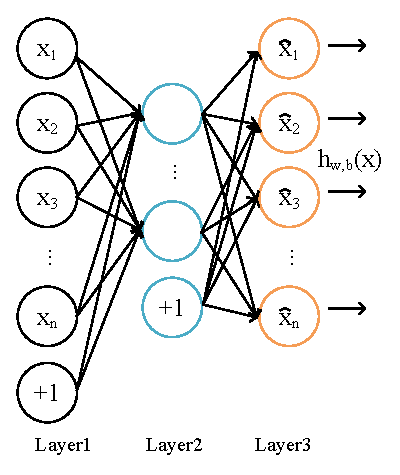
\includegraphics[width=0.58\linewidth]{figures/autoencoder.eps}
\caption{Representation of an autoencoder~\cite{Ng01}}
\label{fig:autoencoder}
\end{figure}

\subsection{Deep Neural Networks with Sparse Autoencoders}
An autoencoder neural network is an unsupervised learning algorithm
that makes use of backpropagation, setting the targets values to be
equal to the inputs.

Using deep sparse autoencoder (DSAE) can learn high-level features
of the input data effectively. Each Sparse Autoencoder in a DSAE can
learn features at different levels (from low level to high level). A
representation of this architecture is shown in
Figure~\ref{fig:deep_neural_network}.

\begin{figure}
\centering
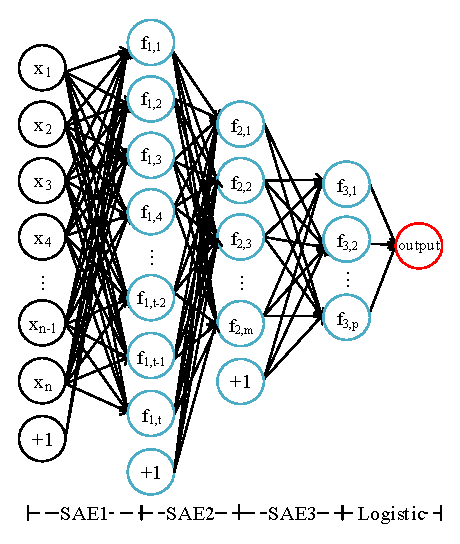
\includegraphics[width=0.8\linewidth]{figures/deep_neural_architecture.eps}
\caption{Deep Neural Network representation,
composed of three SAEs as the hidden layers~\cite{DNN}}
\label{fig:deep_neural_network}
\end{figure}

\section{Proposal} \label{Proposal}
This work is inspired by the work of~\cite{DNN} by the use of
sparse autoencoders as the regression model in order to learn features
from local and global information generated from a human-annotated
keypoint database. Also this proposal is influenced by~\cite{UnsLearning},
so for us to achieve the 3-D keypoint detection we train a 3-layered locally
connected sparse autoencoder similarly to their technique, such
technique's results revealed to be a inexpensive way to develop
high-level features from unlabeled data, from that study this work
presents an adapted architecture for 3-D meshes. Taking a different approach
than the other techniques mentioned above, resized and simplified segments
of the 3-D mesh will be used as the input for our Deep Neural Network,
this will enable our DNN to learn when one of these segments has inside
a keypoint.

\subsection{Mesh Simplification}
One of the objectives of this research is to reduce the amount of data
that is processed to detect 3-D keypoints, to accomplish that we propose 
to simplify the input our Deep Neural Network receives. Several approaches
have been proposed and discussed, we make use of Mesh Saliency's
approach~\cite{Lee01}: Guide the simplification proccess through mesh
curvature obtained from local areas using a center-surround mechanism
to identify regions that are different from their local context. An example
is seen in Figure~\ref{fig:simplification}.

\begin{figure}
\centering
\includegraphics[width=1\linewidth]{figures/mesh_simplification.png}
\caption{Saliency-based weights and quality of a 99\% simplification
for three choices of the simplification weights: (a) Original mesh saliency,
(b) amplified mesh saliency and (c) smoothed and amplified mesh saliency~\cite{Lee01}}
\label{fig:simplification}
\end{figure}  

\subsection{Architecture}
This technique can be seen as a set of sparse deep autoencoders that
similarly to~\cite{UnsLearning} has two fields in it: local receptive fields,
pooling normalization (the architecture taken as a base can be seen
on the Figure~\ref{fig:architecture}). Local receptive fields scale the
autoencoder to big inputs, connecting the autoencoder's features to a small
region of the next lower layer. These sublayers are know as filtering and
pooling.

Originally the neurons in the first sublayer were connected to
pixels in all input channels~\cite{UnsLearning}, but in order to adapt
this architecture it is proposed to use the 3-D vertices and their
connectivity information as the input channels and by so adding more
receptive fields.

\begin{figure}
\centering
\includegraphics[width=0.95\linewidth]{figures/architecture.png}
\caption{Large scale unsupervised learning architecture \cite{UnsLearning}}
\label{fig:architecture}
\end{figure}

\subsection{Training}
As mentioned before the first layer input...

To train the Deep Neural Network what is to be done at first is to train each
Sparse Autoencoder and a final logistic regression layer, then following the
schema from~\cite{DNN} stack the four layers together and backpropagate the
whole DNN to fine tune it.

The goal of this approach is to reduce the proccessing that is performed,
instead of evaluating each vertex in the DNN which is expensive, we can
perform the neccesary calculations just for some samples of the 3-D object
and discard if those samples don't contain any keypoints, in the case we find
the presence of keypoints we will perform further calculations to choose the
sample keypoint.

\section{Results} \label{Results}

\section{Conclusions} \label{Conclusions}

\ack{This research was undertaken as part of the motivation received
from my family and future wife that I probably met already.}


\nocite{*}

\bibliographystyle{compj}
% \bibliography{ModellingBidders}
\input{sample.bbl}


\end{document}
